%----------------------------------------------------------------------------------------
%	Capítulo 3
%----------------------------------------------------------------------------------------

\newpage
\clearpage{\pagestyle{empty}\cleardoublepage}
\doublespacing
%% NUEVO CAPITULO X
\chapter{Título del capítulo 3}
\newpage
\pagestyle{myportland}

%% NUEVA SECCIÓN X.X
\section{Título de sección 1}

Así se cita una página en específico o un rango
Página:

\cite[p.~159]{Pahl2007}

Rango de páginas:

\cite[p.~159-165]{Pahl2007}

%% NUEVO SUBSECCION X.X.X
\subsection{Título de subsección 3}

Contenido


%% NUEVA SUB-SUB-SECCION X.X.X.X
\subsubsection{Tabla compleja que mantiene encabezado y pies de página}

\begin{savenotes}
	% Please add the following required packages to your document preamble:
	% \usepackage{multirow}
	% \usepackage[table,xcdraw]{xcolor}
	% If you use beamer only pass "xcolor=table" option, i.e. \documentclass[xcolor=table]{beamer}
	% \usepackage{longtable}
	% Note: It may be necessary to compile the document several times to get a multi-page table to line up properly
	\scriptsize
	\begin{longtable}{|c|p{0.6cm}|p{10cm}|c|}		
		\caption{Resumen de los requerimientos del sistema.}
		\label{tab:resumen de los requerimientos del sistema}\\
		\hline
		\rowcolor[HTML]{A6A6A6} 
		\multicolumn{4}{|c|}{\cellcolor[HTML]{A6A6A6}{\color[HTML]{000000} \textbf{LISTA DE REQUERIMIENTOS}}} \\ \hline
		\endfirsthead
		%
		\multicolumn{4}{c}%
		{{Tabla \thetable\ continuación de la anterior página.}} \\
		\hline
		\rowcolor[HTML]{A6A6A6} 
		\multicolumn{4}{|c|}{\cellcolor[HTML]{A6A6A6}{\color[HTML]{000000} \textbf{LISTA DE REQUERIMIENTOS}}} \\ \hline
		\rowcolor[HTML]{D9D9D9} 
		\textbf{PROYECTO} &
		\multicolumn{2}{c|}{\cellcolor[HTML]{D9D9D9}\textbf{\begin{tabular}[c]{@{}c@{}}DISEÑO DE CLASIFICADORA Y CONTADORA\\  DE TRUCHAS ARCOÍRIS (Oncorhynchus mykiss)\\ DE 10 A 20 CM. PARA LA CRIANZA DE TRUCHAS\\ EN LA LAGUNA DE PAUCARCOCHA\end{tabular}}} &
		\textbf{\begin{tabular}[c]{@{}c@{}}Fecha:\\ 2020-05-07\\ Página 1 de 1\end{tabular}} \\ \hline
		\rowcolor[HTML]{D9D9D9} 
		{\color[HTML]{000000} \textbf{\begin{tabular}[c]{@{}c@{}}Última \\ modificación\end{tabular}}} &
		{\color[HTML]{000000} \textbf{\begin{tabular}[c]{@{}c@{}}D/\\ E\end{tabular}}} &
		\multicolumn{1}{c|}{\cellcolor[HTML]{D9D9D9}{\color[HTML]{000000} \textbf{Requerimientos}}} &
		{\color[HTML]{000000} \textbf{Reponsable}} \\ \hline
		\endhead
		%
		\rowcolor[HTML]{D9D9D9} 
		\textbf{PROYECTO} &
		\multicolumn{2}{c|}{\cellcolor[HTML]{D9D9D9}\textbf{\begin{tabular}[c]{@{}c@{}}DISEÑO DE CLASIFICADORA Y CONTADORA\\  DE TRUCHAS ARCOÍRIS (Oncorhynchus mykiss)\\ DE 10 A 20 CM. PARA LA CRIANZA DE TRUCHAS\\ EN LA LAGUNA DE PAUCARCOCHA\end{tabular}}} &
		\textbf{\begin{tabular}[c]{@{}c@{}}Fecha:\\ 2020-05-07\\ Página 1 de 1\end{tabular}} \\ \hline
		\rowcolor[HTML]{D9D9D9} 
		{\color[HTML]{000000} \textbf{\begin{tabular}[c]{@{}c@{}}Última \\ modificación\end{tabular}}} &
		{\color[HTML]{000000} \textbf{\begin{tabular}[c]{@{}c@{}}D/E\footnote{Deseo (D) y exigencia (E).}\end{tabular}}} &
		\multicolumn{1}{c|}{\cellcolor[HTML]{D9D9D9}{\color[HTML]{000000} \textbf{Requerimientos}}} &
		{\color[HTML]{000000} \textbf{Reponsable}} \\ \hline
		
		
					&    & \underline{Función principal:}																										& P.D.V. 	\\
		2019-09-24  & E  & Clasificar y contar truchas arcoíris de 10 a 20 $ cm $. en al menos 2 salidas y enviar un reporte de la clasificación y el conteo.   & \multicolumn{1}{l|}{}	\\ 
					&    & \underline{Geometría:}																												& \multicolumn{1}{l|}{}	\\
		2019-09-24  & E  & El sistema no debe exceder los 200x200x200 $ cm $.																					& \multicolumn{1}{l|}{}	\\ 
					&    & \underline{Fuerzas:}																													& \multicolumn{1}{l|}{}	\\
		2019-09-24  & E  & Pesar menos de 200 $ kg $.																											& \multicolumn{1}{l|}{}	\\ 
					&    & \underline{Energía:}																													& \multicolumn{1}{l|}{}	\\
		2019-10-05  & E  & Usará baterías DC.																													& \multicolumn{1}{l|}{}	\\ 	
		2019-09-24  & E  & Funcionar desde -10 a 40 °C.																											& \multicolumn{1}{l|}{}	\\ 	
		2019-09-24  & D  & La máquina debe enviar la información.																								& \multicolumn{1}{l|}{}	\\ 	
					&    & \underline{Materiales:}																												& \multicolumn{1}{l|}{}	\\
		2019-09-22  & E  & La máquina debe ser inoxidable.																										& \multicolumn{1}{l|}{}	\\ 	
		2019-09-20  & E  & La máquina no debe desprender ningún residuo que pueda contaminar el agua.															& \multicolumn{1}{l|}{}	\\ 	
		2019-09-25  & D  & Los materiales de manufactura deben poder ser adquiridos en el mercado peruano.														& \multicolumn{1}{l|}{}	\\ 			
					&    & \underline{Señales:}																													& \multicolumn{1}{l|}{}	\\
		2019-09-24  & E  & Se debe enviar una señal en caso de fallo del sistema y pausar el proceso.															& \multicolumn{1}{l|}{}	\\ 	
					&    & \underline{Hardware:}																												& \multicolumn{1}{l|}{}	\\
		2019-10-05  & E  & La máquina debe usar cámaras o dispositivos similares para obtener imágenes.															& \multicolumn{1}{l|}{}	\\ 		
					&    & \underline{Software:}																												& \multicolumn{1}{l|}{}	\\
		2019-10-05  & D  & El sistema generará un reporte de la clasificación y conteo.																			& \multicolumn{1}{l|}{}	\\ 	
					&    & \underline{Costos:}   																												& \multicolumn{1}{l|}{}	\\ 
		2019-09-24  & D  & El precio unitario menor a 10 mil dólares.       								    												& \multicolumn{1}{l|}{}	\\  \hline
		
		
		\rowcolor[HTML]{D9D9D9} 
		\multicolumn{1}{|l|}{\cellcolor[HTML]{D9D9D9}{\color[HTML]{000000} }} &
		\multicolumn{2}{c|}{\cellcolor[HTML]{D9D9D9}{\color[HTML]{000000} \textbf{Última modificación: 2019-10-05}}} &
		{\color[HTML]{000000} } \\ \hline
	\end{longtable}

\end{savenotes}

%% NUEVO SUBSECCION X.X.X
\subsection{Cambiar la página a horizontal}

Contenido, se debe ajustar el width para que pueda entrar el número de la página

\newpage
\thispagestyle{mylandscape}
\begin{landscape}
	\begin{figure}[H]
		\centering
		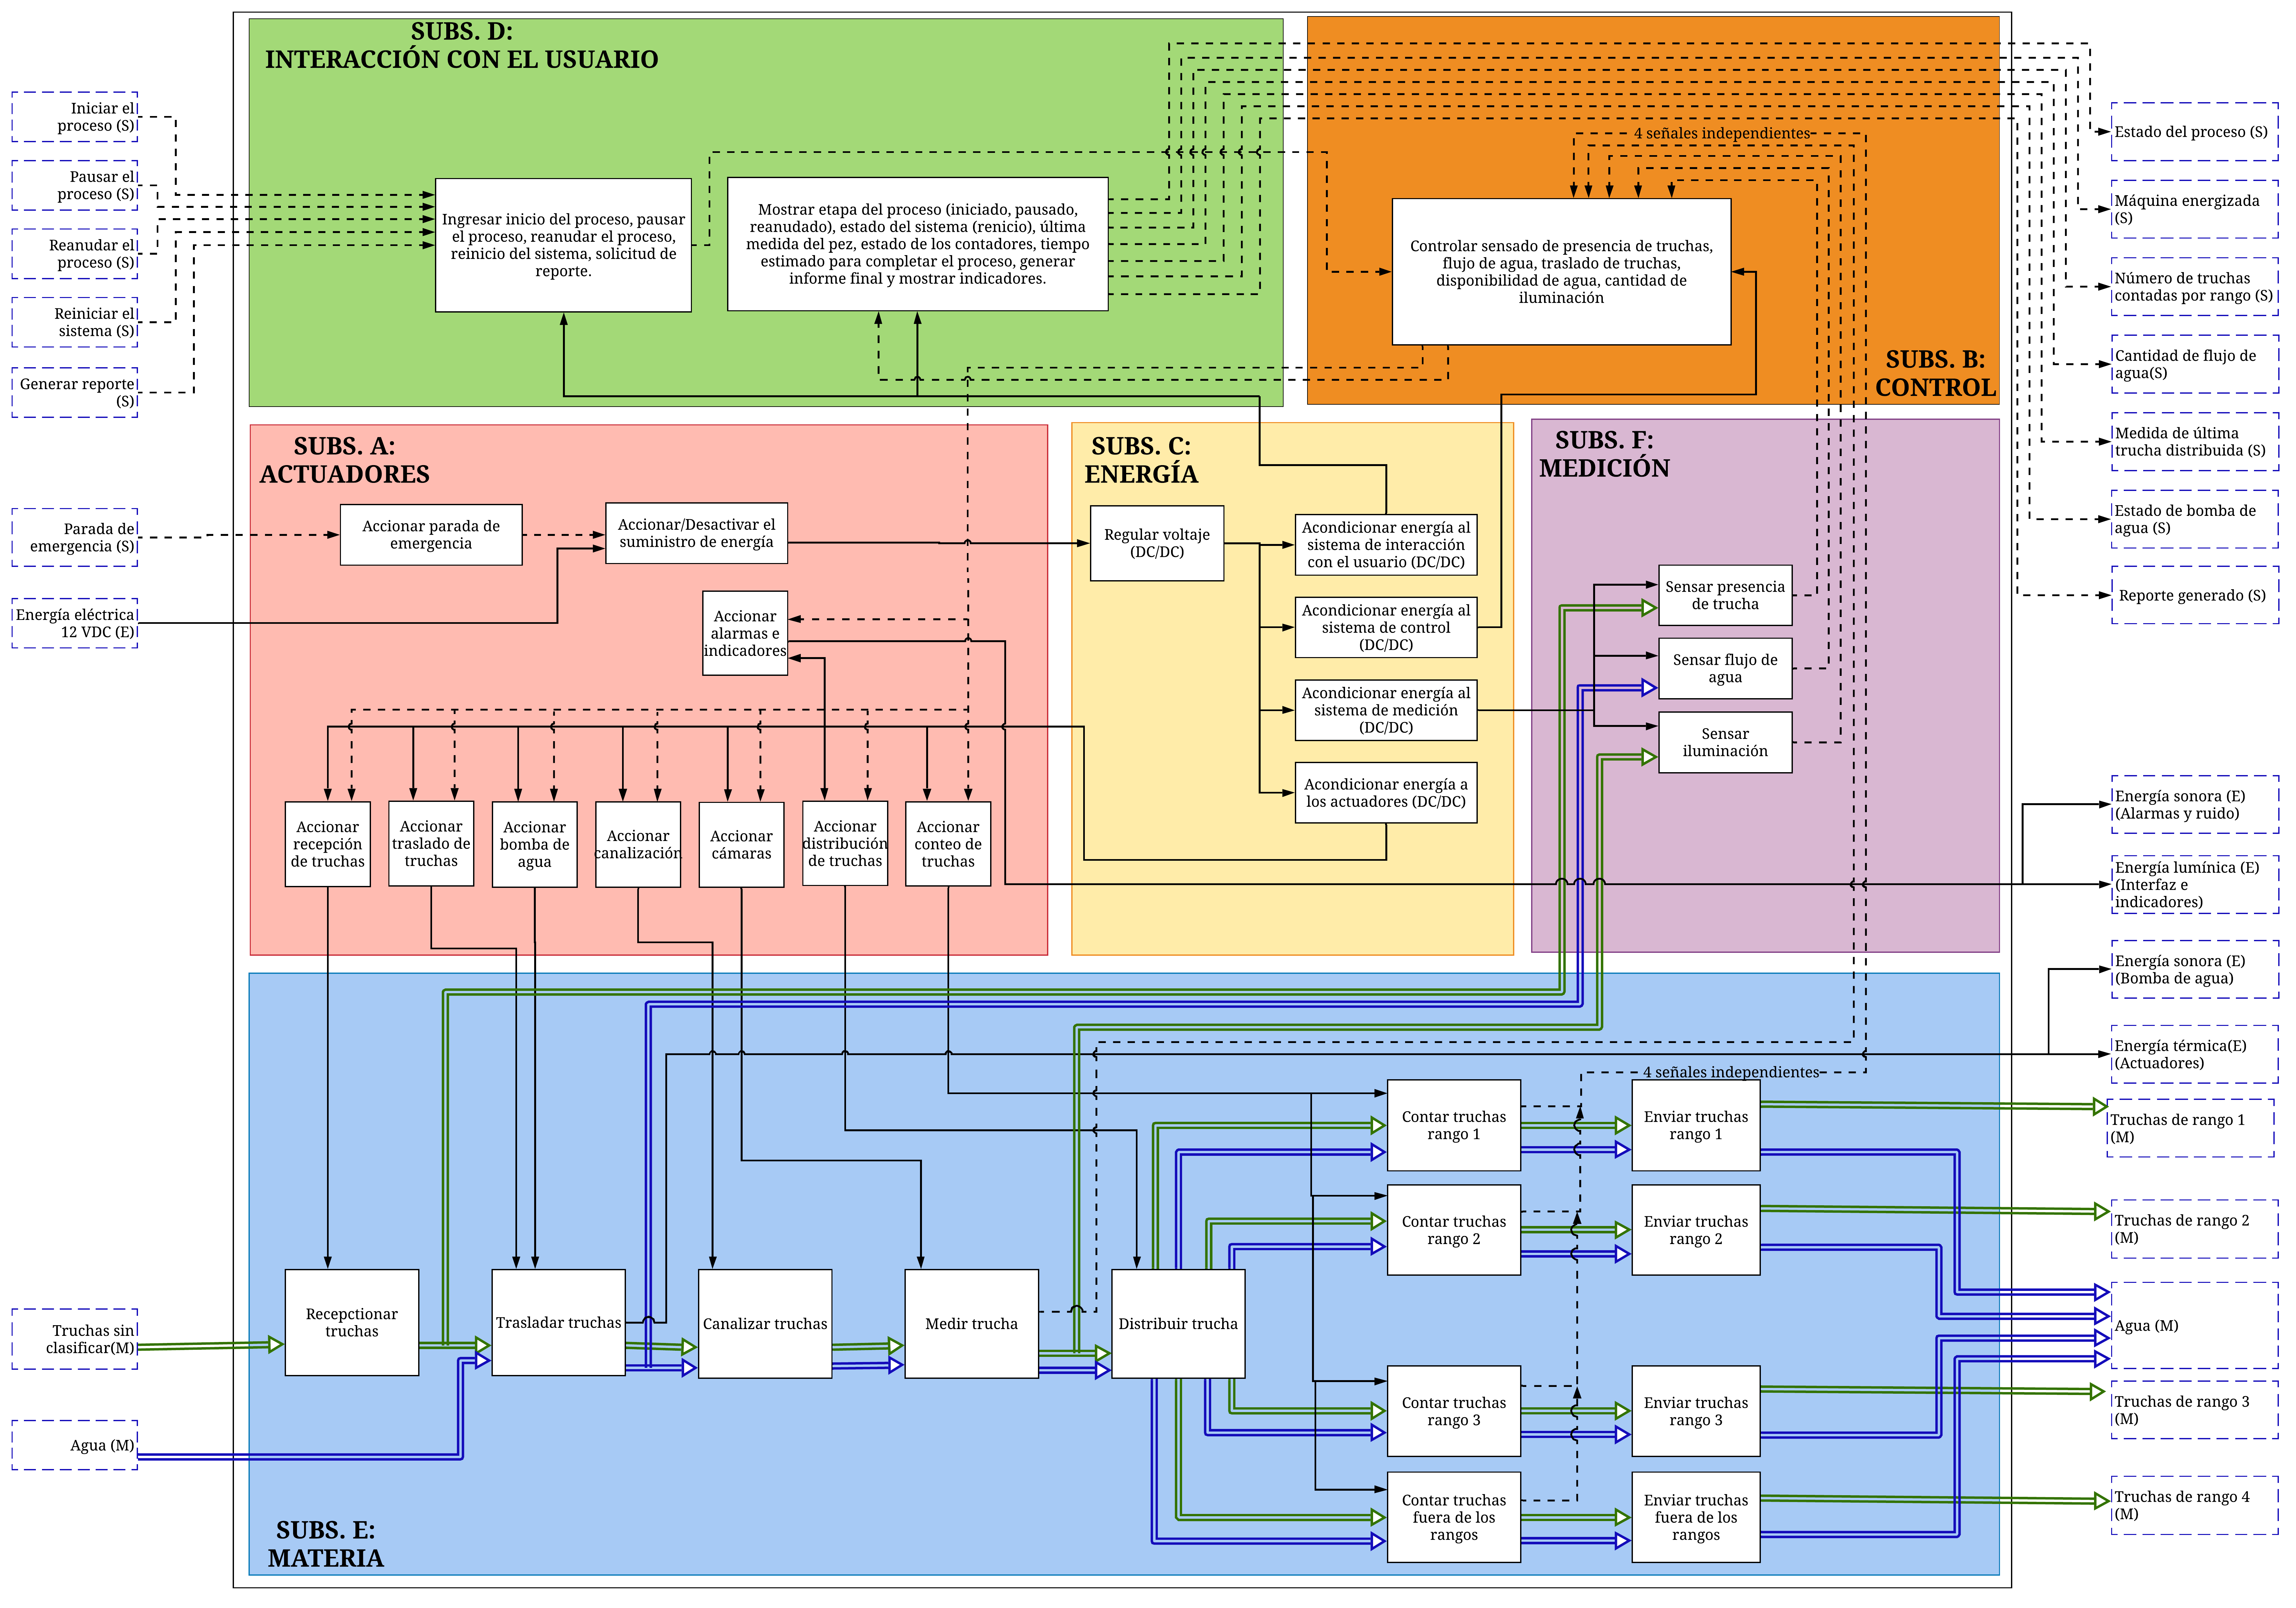
\includegraphics[width=0.98\paperwidth]{chapter3/estructura global de funciones.png}
		\caption{Estructura global de funciones.}
		Fuente: Elaboración propia.
		\label{fig:estructura global de funciones}
	\end{figure}
\end{landscape}


\newpage
\thispagestyle{fancy}

Aquí ya devolví el formato a vertical

%% NUEVA SUB-SUB-SECCION X.X.X.X
\subsubsection{Cómo hacer una lista}

Así se hace una lista

\begin{enumerate}
	
	\item Item nivel 1
		
		\begin{enumerate}[label=\Alph*)] % \alph for lowercase
			\item	\textbf{Item nivel 2} Descripción
			
			\item	\textbf{Item nivel 2} Descripción			
			
		\end{enumerate}
	
	\item Item nivel 1
		
		\begin{enumerate}[label=\Alph*)] % \alph for lowercase
			\item	\textbf{Item nivel 2} Descripción
			
			\item	\textbf{Item nivel 2} Descripción			
			
		\end{enumerate}
	
	%	To create new enumerate alpha use code below
	%	\begin{enumerate}[label=\Alph*)] % \alph for lowercase
	%	\end{enumerate}
\end{enumerate}



\newpage
\pagestyle{mylandscape}

\begin{landscape}
	\begin{figure}[H]
		\centering
		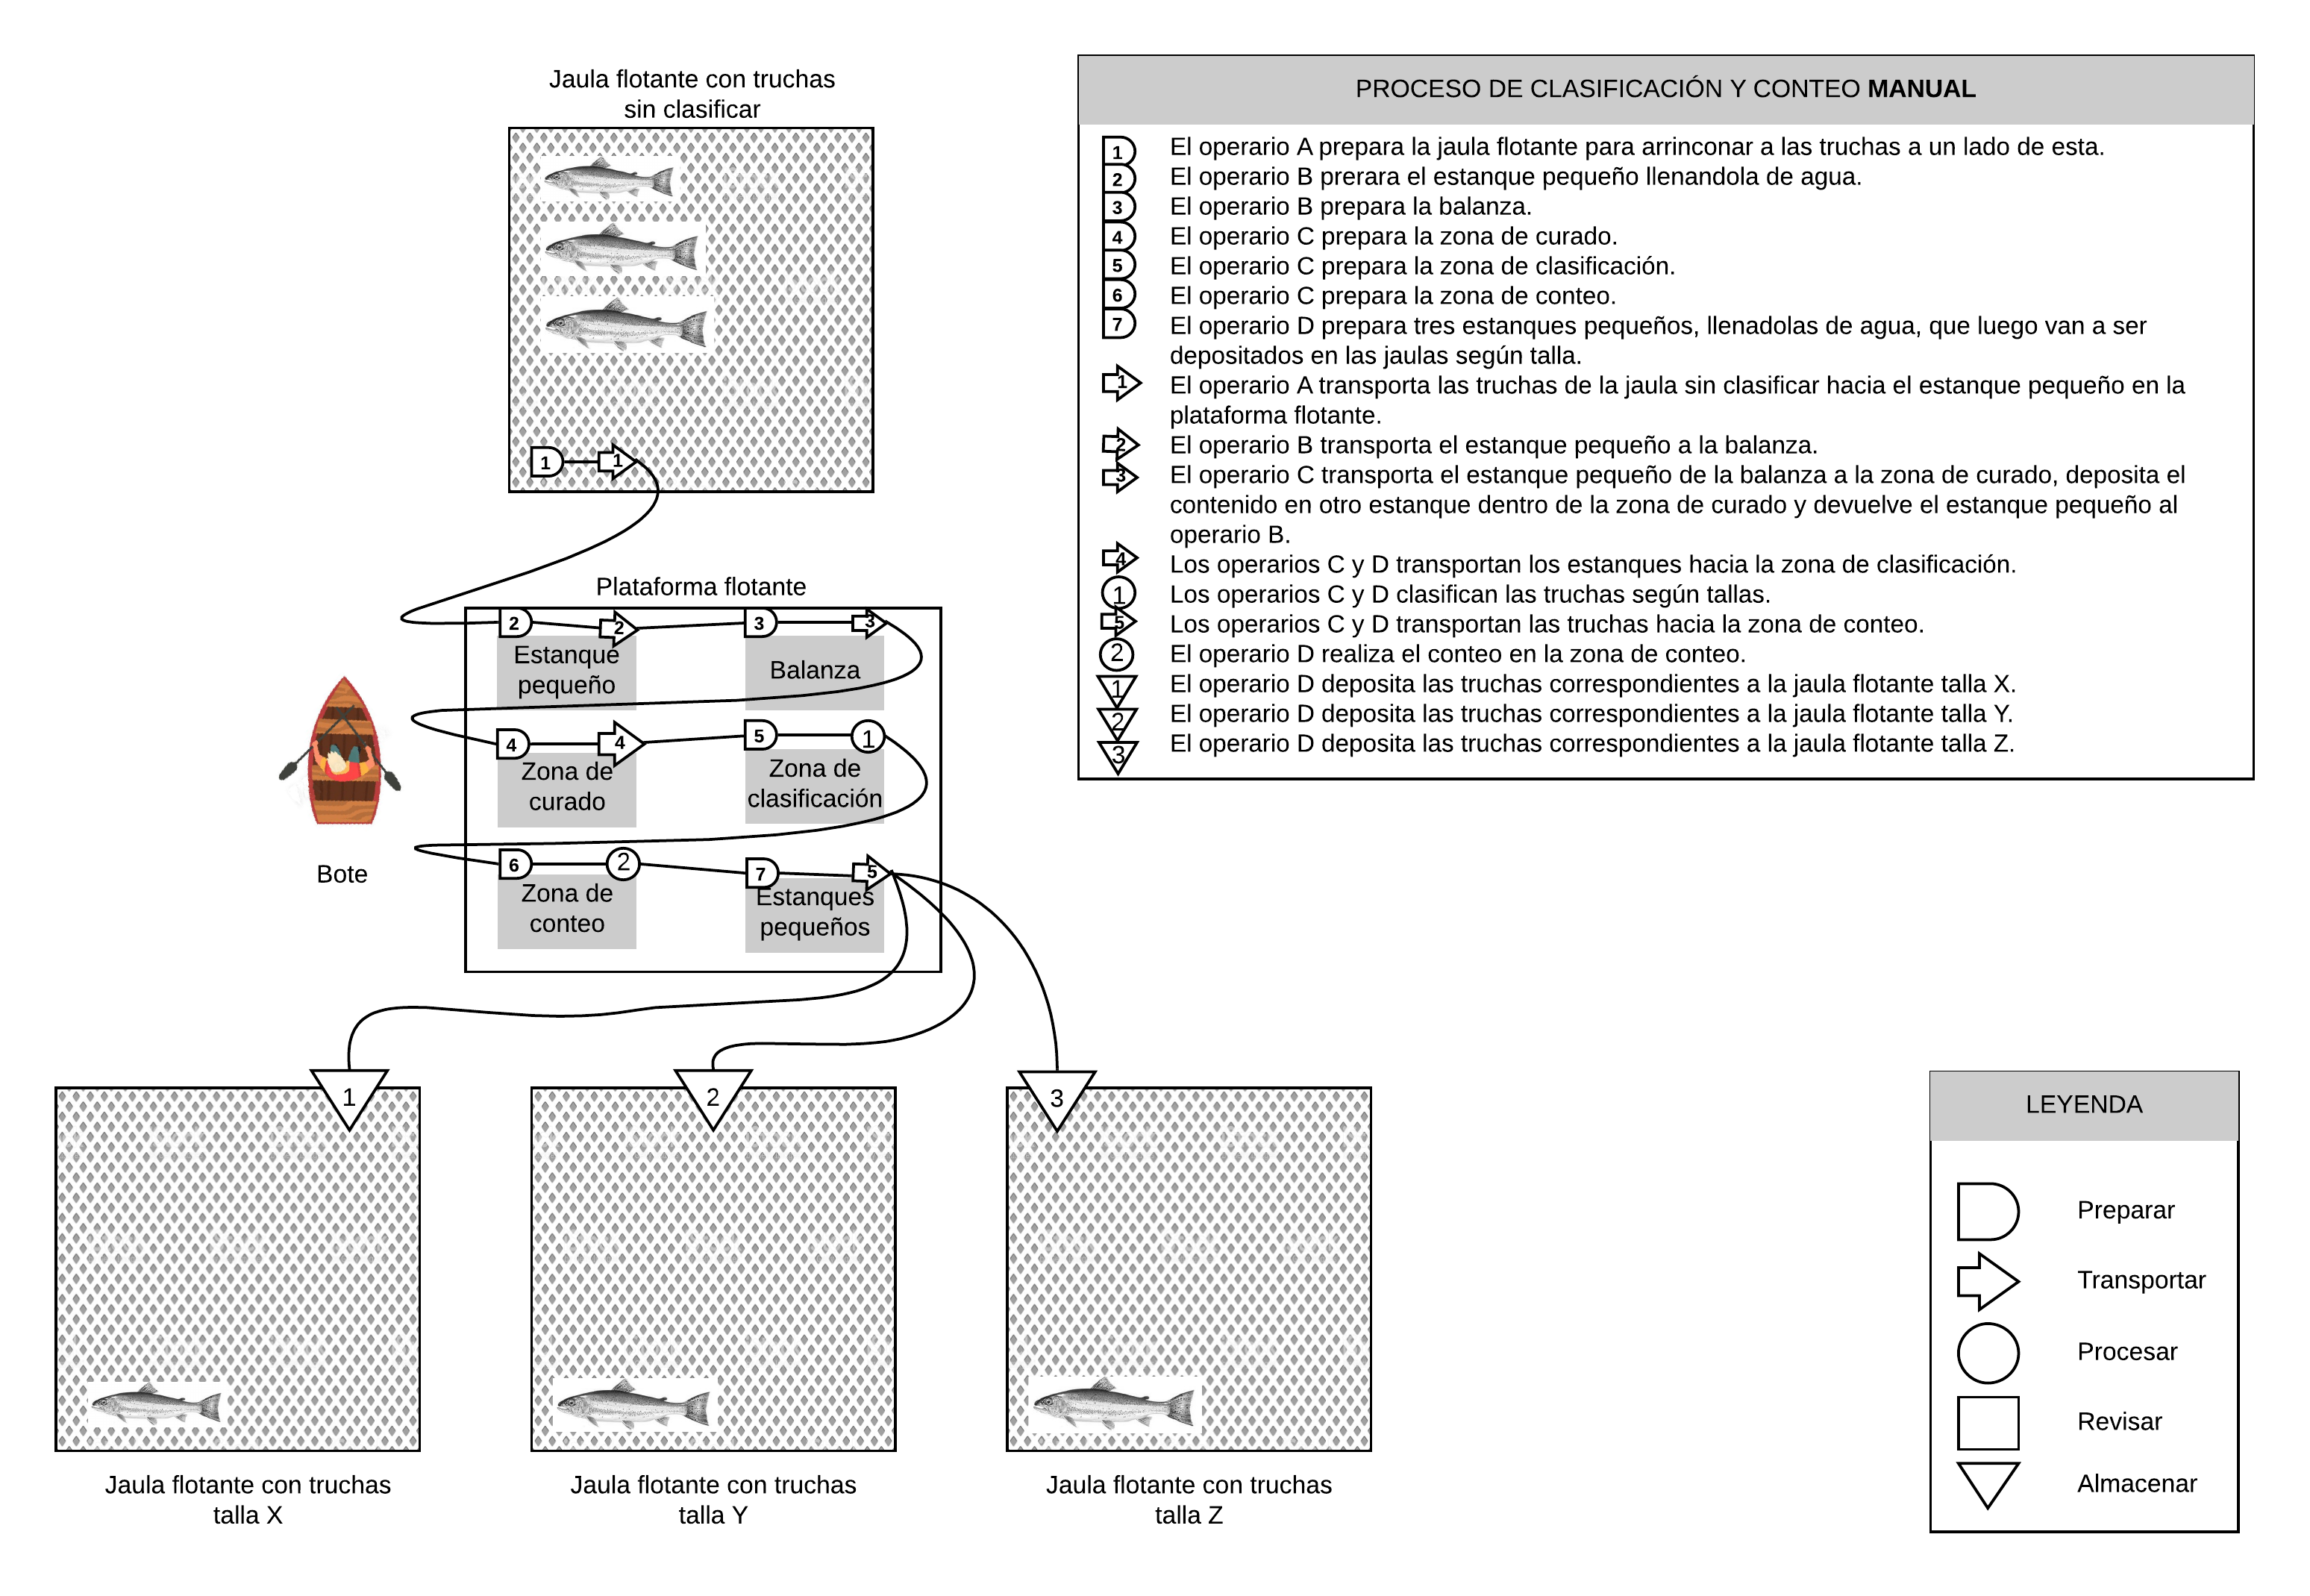
\includegraphics[width=0.98\paperwidth]{chapter3/proceso de clasificacion y conteo manual.png}
		\caption{Método manual de clasificación y conteo de truchas.}
		Fuente: Elaboración propia.
		\label{fig:proceso de clasificacion y conteo manual}
	\end{figure}
\end{landscape}

\newpage
\pagestyle{fancy}
